\subsection{Self-Organizing Map Algorithm}\label{ssec:som}

Self-organizing map is only a slight variant of vector quantization
explained in Section~\ref{ssec:cl}.
The key idea is that lateral interactions of the nodes is crucial
for the nodes to learn in a dependent fashion;
that is, the nodes are treated as a \emph{topologically related subset}
for which the learning or update is enforced similarly for nodes which are close.
SOM defines this lateral interaction using a neighborhood set $N_c$ of the node $c$
where $m_c = \argmin\limits_{m \in \set{m_i}} \norm{x-m_i}$.
We call $m_c$ the \emph{best-matching unit} (BMU).
$N_c$ is essentially a ball in the node-space
and is completely defined by the node $c$ and a radius.
Experiments show that adaptively changing this radius,
in particular, starting with a large radius and gradually decreasing it,
is advantageous for the learning process.
A heuristic argument is that a large radius first captures
some global order of the $m_i$ codebook vectors
and are afterwards refined to a local order.

The codebook vector update is as follows:
\begin{align*}
    m_i(t+1)
    &=
    \begin{cases}
        m_i(t) + \alpha(t) (x(t) - m_i(t)) ,& i \in N_c(t) \\
        m_i(t),& i \notin N_c(t)
    \end{cases}
    =
    m_i(t) + h_{c,i}(t) (x(t) - m_i(t))
    \\
    h_{c,i}(t)
    &=
    \begin{cases}
        \alpha(t) ,& i \in N_c(t) \\
        0 ,& i \notin N_c(t)
    \end{cases}
\end{align*}
where $\alpha(t)$ is the learning-rate as in Section~\ref{ssec:cl}.
The kernel $h_{c,i}(t)$ is called the Bubble neighborhood function.
As an analogy to KNN, this kernel can be considered as a hard-thresholding weight function.
Another popular neighborhood function is the Gaussian,
which draws a larger parallel to biological lateral interaction,
$h_{c,i}(t) := h_0(t) \exp\paren{-\norm{r_i-r_c}^2 / \sigma(t)^2}$
where $r_i, r_c$ are the coordinates of the nodes $i, c$
and $h_0(t), \sigma(t)$ are suitable decreasing functions of time.

Letting $N$ be the number of iterations,
the complete SOM algorithm is outlined below:

\begin{algorithm}[H]
\SetAlgoLined
Randomly initialize the codebook vectors\;
\While{$j < N$} {
    Randomly pick an input vector $x$\;
    Compute the BMU $m_c$\;
    \For{i in $N_c$}{
        $m_i = m_i + \alpha h_{c,i} (x - m_i)$\;
    }
}
\caption{SOM algorithm}
\end{algorithm}

\begin{figure}[t]
    \centering
    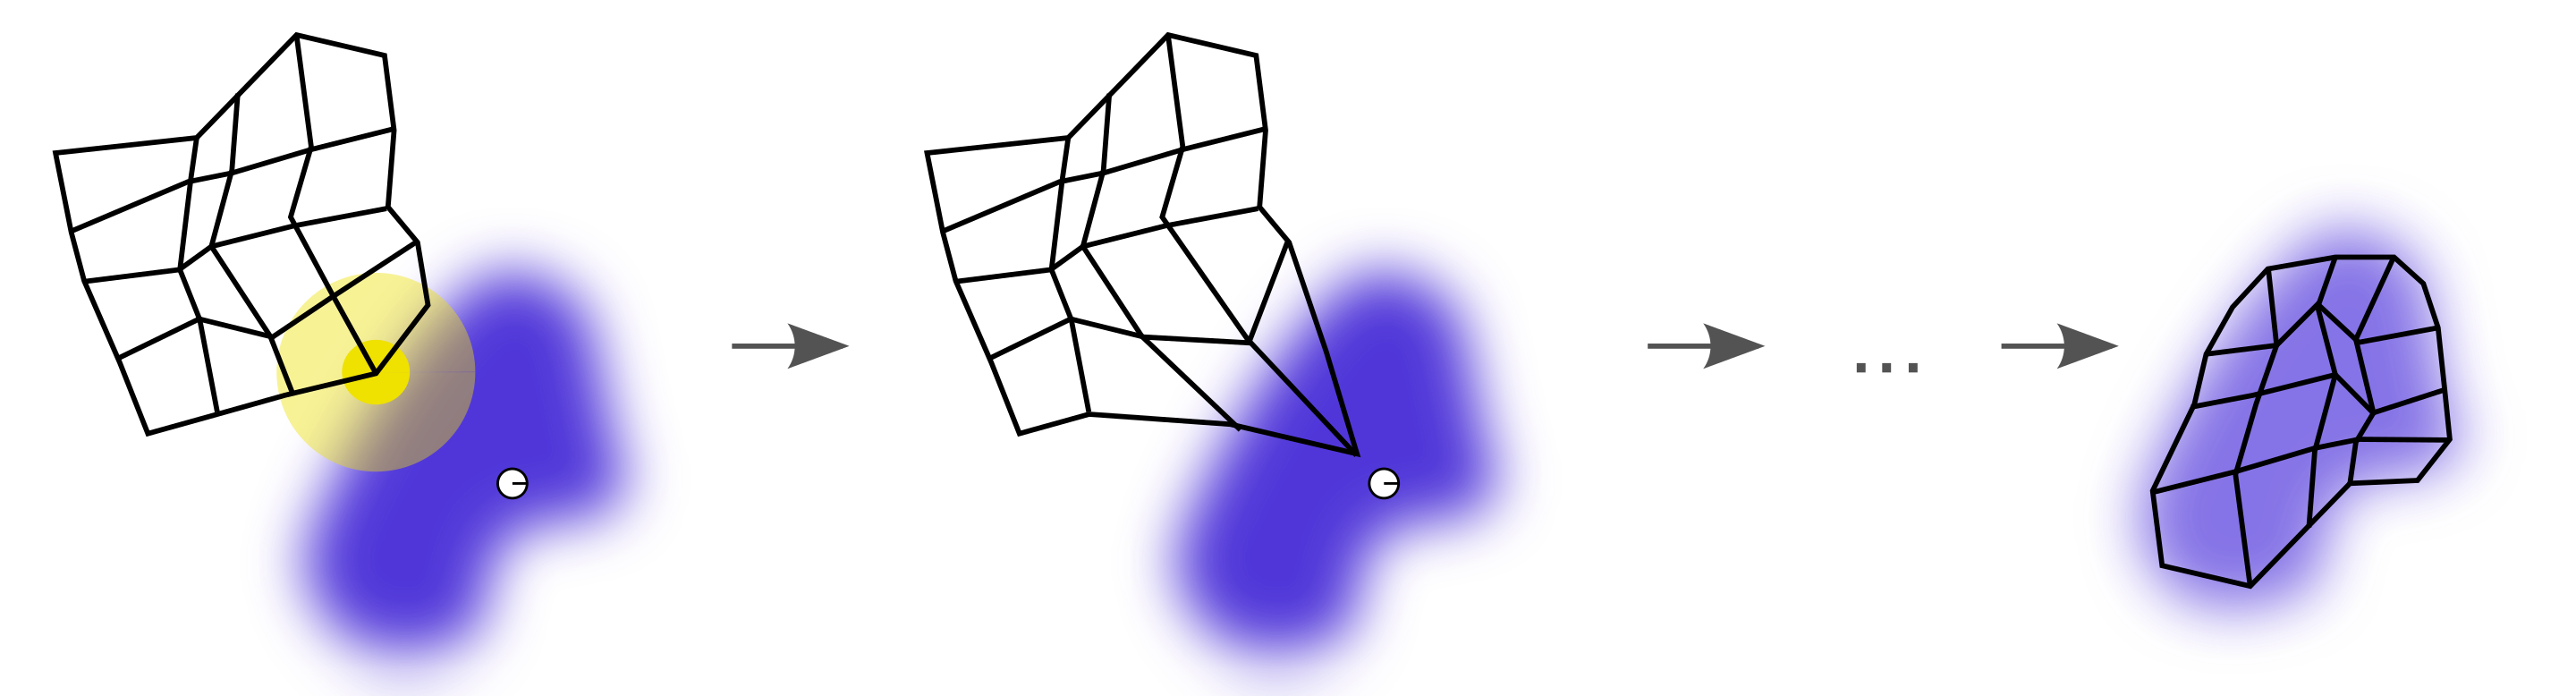
\includegraphics[width=\textwidth]{../figs/som-training.png}
    \caption{An illustration of SOM training.}
    \label{fig:som-training}
\end{figure}

Figure~\ref{fig:som-training} shows an illustration of SOM training~\cite{som-training:2010}.
The manifold represents the two-dimensional grid of nodes.
The blue patch is the input space where the data lives
and the white circle on the blue patch is the current sample we randomly picked.
The first picture shows a yellow highlight, which represents the BMU\@.
The second picture shows the node moving closer to the current sample via the update rule.
Finally, after many iterations, the last picture shows the final configuration
of the nodes where each node becomes sensitive to a certain aspect of the data.
